\chapter{Versuch 2}

\section{Benötigte Geräte}

Für dieses Experiment benötigen wir die Folgenden Geräte:

\begin{tabular}[h]{c|c|c}
    Gerät & Anzahl & Produktbeeichnung\\
    \hline
    Oszilloskop & 1  & Keysight DSOX1102A\\
    \hline
    Frequenzgenerator & 1 & TELEDYNE T3AFG80\\
	\hline 
	Digital-Multimeter & 1 & Fluke TRUE RMS MULTIMETER\\
	\hline
	DAC & 1 & ZN429E \\
	\hline
	D-Flip-Flop & 1 & \\
	\hline
    \label{tab:Materialliste Versuch 2}
\end{tabular}


\section{Versuchsaufbau}
\begin{figure}[H]
	\centering
	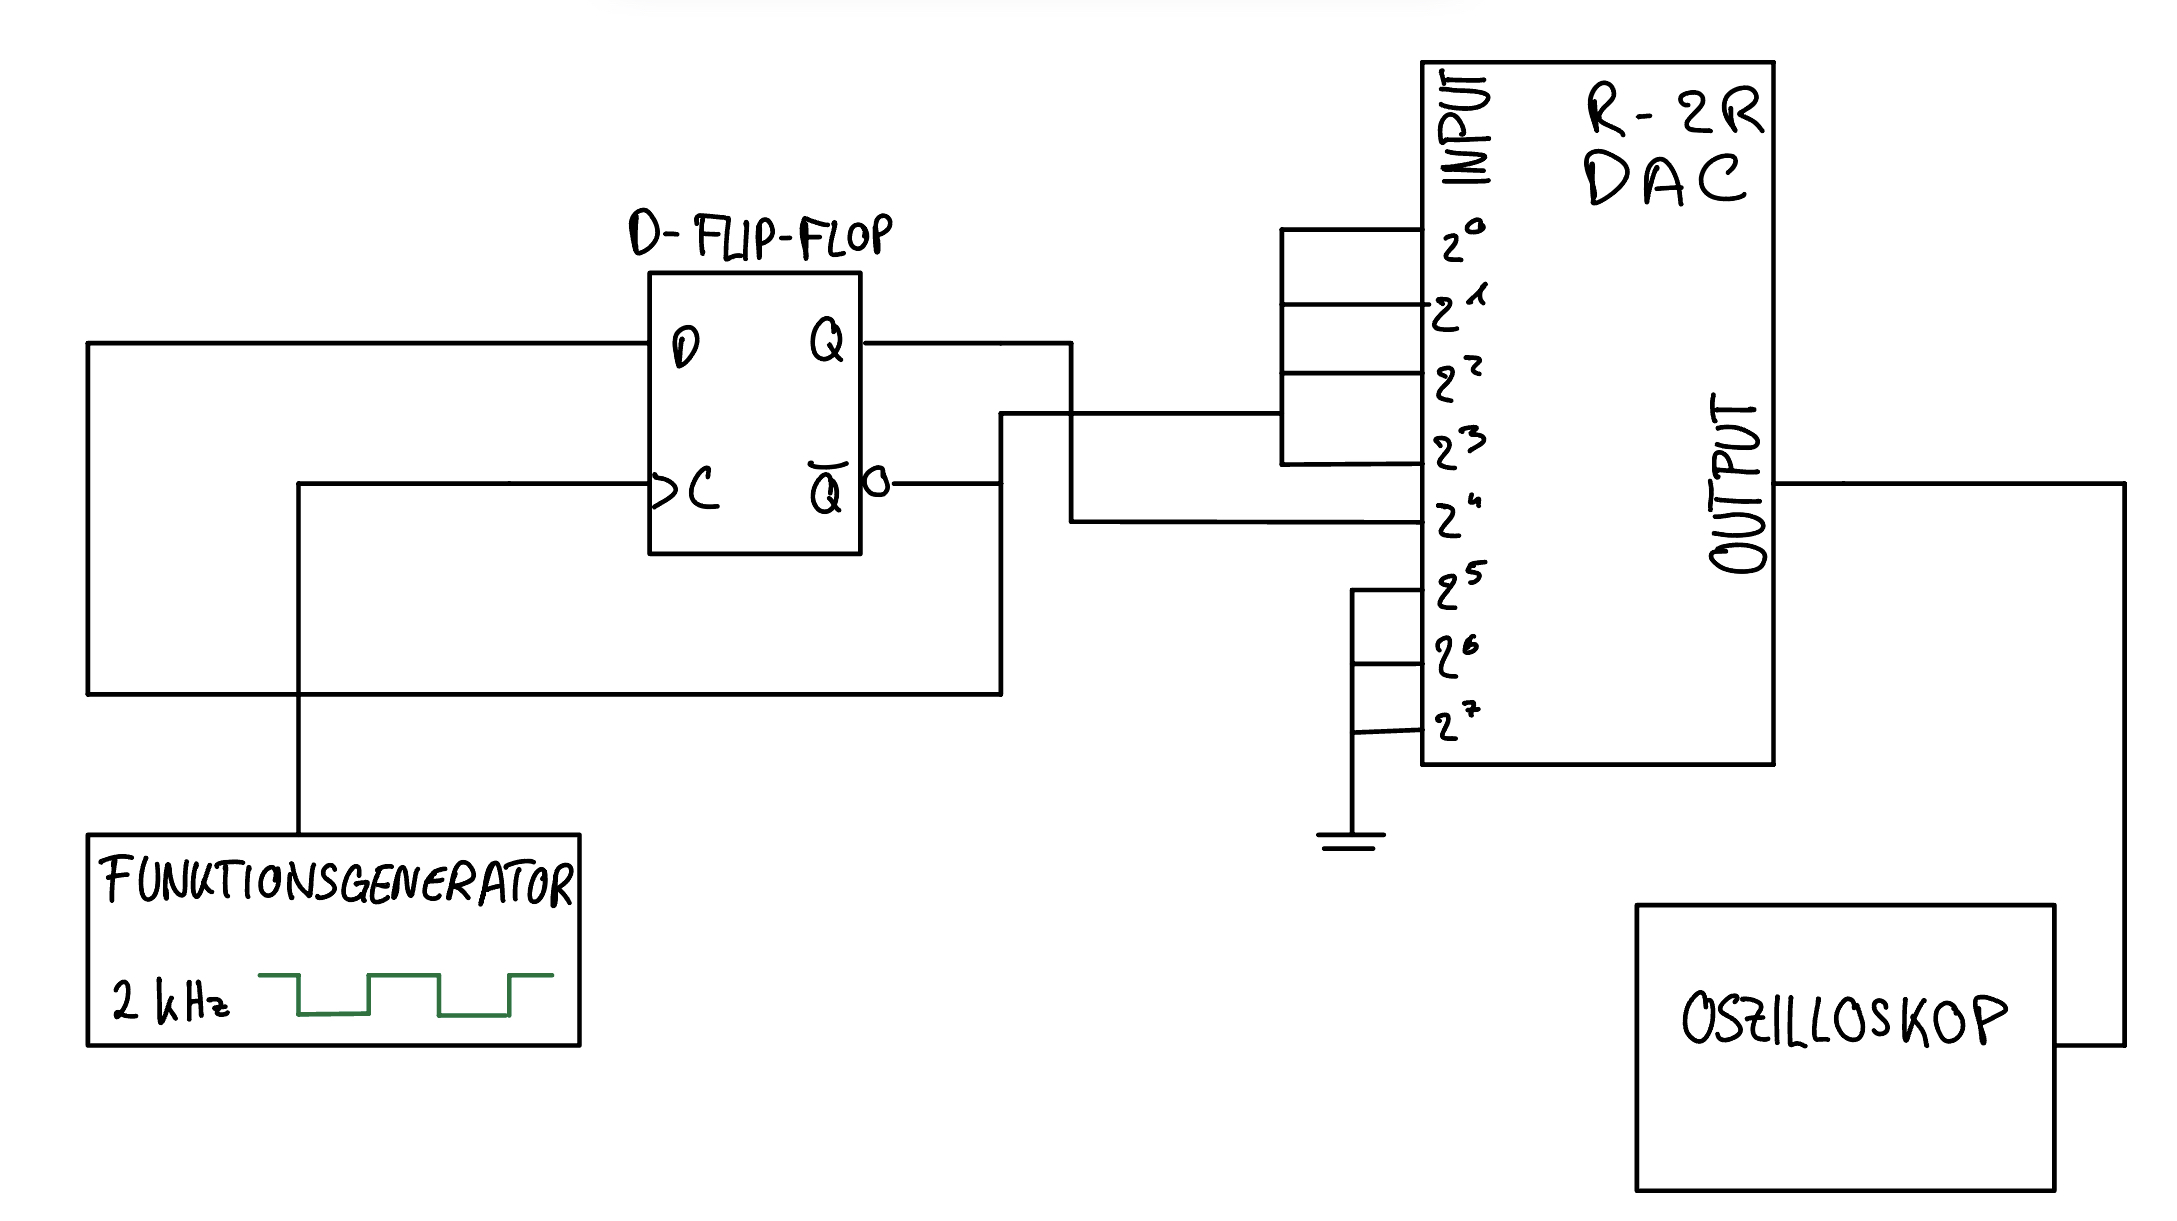
\includegraphics[height=7cm]{images/schaltungsskizze-versuch-zwei.jpeg} 
	\caption[]{Schaltungsskizze Versuch 2}
\end{figure}
Durch die Verbindung von D mit !Q erreichet man eine aufsteigende Flanke
in einem Interval von 0,1ms. 

XXXXXXXXXXXXX Vref wurde angegeben

XXXXXXXXXXXXX Kondesator brauch man nicht.

\section{Monotonie und Nichtlinearität}
einfügen excel tabelle
erklären 5. Bit kaputt


Aus dem Datenblatt kann man ablesen, dass die Ausgangsimpedanz vom
DAC 10k$\Omega$ beträgt.



\section{Einschwingverhalten}

Zunächst einmal wurde der defekte DAC ausgetauscht 
gegen einen voll-funktionsfähigen. \newline

Die Frequenz der Alternierung des Flip-Flops ändert man zunächst nicht. \newline

Zum messen des Einschwingverhaltens legt man 2 Bitsprünge fest.
Einerseits den Bitsprung von 0000 0000 -> 0000 0001 und andererseits 
den Bitsprung von 0000 0000 -> 1111 1111.
Diese Werte eigenen sich gut, da hier im Datenblatt vom Hersteller 
zwei Referenzwerte gegeben sind, welche man nun zum Vergleich verwenden kann.\newline

Als Scope am Oszilloskop stellt man 200ns/div ein. \newline


\begin{tabular}[h]{c|c}
    Bitsprung & Einschwingzeit \\
    \hline
    00000 0000 -> 0000 0001 & 540ns\\
    \hline
    0000 0000 -> 1111 1111 & 800ns \\

\end{tabular}

